\documentclass[tikz,border=5pt]{standalone}
\begin{document}
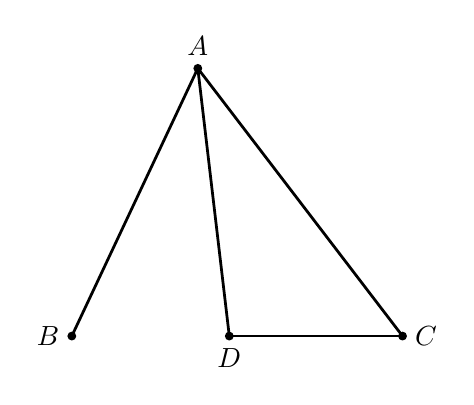
\begin{tikzpicture}[line cap=round,line join=round]
  \coordinate (A) at (1.6,3.4);
  \coordinate (B) at (0,0);
  \coordinate (C) at (4.2,0);
  \coordinate (D) at (2.0,0);

  \draw[line width=1pt] (A) -- (B);
  \draw[line width=1pt] (A) -- (C);
  \draw[line width=1pt] (A) -- (D);
  \draw[line width=1pt] (D) -- (C);

  \fill (A) circle (1.6pt);
  \fill (B) circle (1.6pt);
  \fill (C) circle (1.6pt);
  \fill (D) circle (1.6pt);

  \node[above=1pt] at (A) {$A$};
  \node[left=1pt]  at (B) {$B$};
  \node[right=1pt] at (C) {$C$};
  \node[below=1pt] at (D) {$D$};
\end{tikzpicture}
\end{document}
